\documentclass[9pt,a4paper,]{extarticle}

\usepackage{f1000_styles}

\usepackage[pdfborder={0 0 0}]{hyperref}

\usepackage[numbers]{natbib}


%% maxwidth is the original width if it is less than linewidth
%% otherwise use linewidth (to make sure the graphics do not exceed the margin)
\makeatletter
\def\maxwidth{ %
  \ifdim\Gin@nat@width>\linewidth
    \linewidth
  \else
    \Gin@nat@width
  \fi
}
\makeatother

\usepackage{color}
\usepackage{fancyvrb}
\newcommand{\VerbBar}{|}
\newcommand{\VERB}{\Verb[commandchars=\\\{\}]}
\DefineVerbatimEnvironment{Highlighting}{Verbatim}{commandchars=\\\{\}}
% Add ',fontsize=\small' for more characters per line
\usepackage{framed}
\definecolor{shadecolor}{RGB}{248,248,248}
\newenvironment{Shaded}{\begin{snugshade}}{\end{snugshade}}
\newcommand{\KeywordTok}[1]{\textcolor[rgb]{0.13,0.29,0.53}{\textbf{#1}}}
\newcommand{\DataTypeTok}[1]{\textcolor[rgb]{0.13,0.29,0.53}{#1}}
\newcommand{\DecValTok}[1]{\textcolor[rgb]{0.00,0.00,0.81}{#1}}
\newcommand{\BaseNTok}[1]{\textcolor[rgb]{0.00,0.00,0.81}{#1}}
\newcommand{\FloatTok}[1]{\textcolor[rgb]{0.00,0.00,0.81}{#1}}
\newcommand{\ConstantTok}[1]{\textcolor[rgb]{0.00,0.00,0.00}{#1}}
\newcommand{\CharTok}[1]{\textcolor[rgb]{0.31,0.60,0.02}{#1}}
\newcommand{\SpecialCharTok}[1]{\textcolor[rgb]{0.00,0.00,0.00}{#1}}
\newcommand{\StringTok}[1]{\textcolor[rgb]{0.31,0.60,0.02}{#1}}
\newcommand{\VerbatimStringTok}[1]{\textcolor[rgb]{0.31,0.60,0.02}{#1}}
\newcommand{\SpecialStringTok}[1]{\textcolor[rgb]{0.31,0.60,0.02}{#1}}
\newcommand{\ImportTok}[1]{#1}
\newcommand{\CommentTok}[1]{\textcolor[rgb]{0.56,0.35,0.01}{\textit{#1}}}
\newcommand{\DocumentationTok}[1]{\textcolor[rgb]{0.56,0.35,0.01}{\textbf{\textit{#1}}}}
\newcommand{\AnnotationTok}[1]{\textcolor[rgb]{0.56,0.35,0.01}{\textbf{\textit{#1}}}}
\newcommand{\CommentVarTok}[1]{\textcolor[rgb]{0.56,0.35,0.01}{\textbf{\textit{#1}}}}
\newcommand{\OtherTok}[1]{\textcolor[rgb]{0.56,0.35,0.01}{#1}}
\newcommand{\FunctionTok}[1]{\textcolor[rgb]{0.00,0.00,0.00}{#1}}
\newcommand{\VariableTok}[1]{\textcolor[rgb]{0.00,0.00,0.00}{#1}}
\newcommand{\ControlFlowTok}[1]{\textcolor[rgb]{0.13,0.29,0.53}{\textbf{#1}}}
\newcommand{\OperatorTok}[1]{\textcolor[rgb]{0.81,0.36,0.00}{\textbf{#1}}}
\newcommand{\BuiltInTok}[1]{#1}
\newcommand{\ExtensionTok}[1]{#1}
\newcommand{\PreprocessorTok}[1]{\textcolor[rgb]{0.56,0.35,0.01}{\textit{#1}}}
\newcommand{\AttributeTok}[1]{\textcolor[rgb]{0.77,0.63,0.00}{#1}}
\newcommand{\RegionMarkerTok}[1]{#1}
\newcommand{\InformationTok}[1]{\textcolor[rgb]{0.56,0.35,0.01}{\textbf{\textit{#1}}}}
\newcommand{\WarningTok}[1]{\textcolor[rgb]{0.56,0.35,0.01}{\textbf{\textit{#1}}}}
\newcommand{\AlertTok}[1]{\textcolor[rgb]{0.94,0.16,0.16}{#1}}
\newcommand{\ErrorTok}[1]{\textcolor[rgb]{0.64,0.00,0.00}{\textbf{#1}}}
\newcommand{\NormalTok}[1]{#1}

% disable code chunks background
%\renewenvironment{Shaded}{}{}

% disable section numbers
\setcounter{secnumdepth}{0}


\usepackage{amsthm}
\newtheorem{theorem}{Theorem}
\newtheorem{lemma}{Lemma}
\theoremstyle{definition}
\newtheorem{definition}{Definition}
\newtheorem{corollary}{Corollary}
\newtheorem{proposition}{Proposition}
\theoremstyle{definition}
\newtheorem{example}{Example}
\theoremstyle{remark}
\newtheorem*{remark}{Remark}
\begin{document}
\pagestyle{front}

\title{\emph{F1000Research} Software Tool Article Template}

\author[1]{Nima Hejazi}
\author[2]{Alan E. Hubbard}
\author[2]{Mark J. van der Laan}
\affil[1]{Address of author1}
\affil[2]{Address of author2}

\maketitle
\thispagestyle{front}

\begin{abstract}
Abstracts should be up to 300 words and provide a succinct summary of
the article. Although the abstract should explain why the article might
be interesting, care should be taken not to inappropriately
over-emphasise the importance of the work described in the article.
Citations should not be used in the abstract, and the use of
abbreviations should be minimized.
\end{abstract}

\section*{Keywords}
Please list up to eight keywords to help readers interested in your
article find it more easily.


\clearpage
\pagestyle{main}

\section{Introduction}\label{introduction}

The introduction provides context as to why the software tool was
developed and what need it addresses. It is good scholarly practice to
mention previously developed tools that address similar needs, and why
the current tool is needed.

\section{Methods}\label{methods}

\subsection{Implementation}\label{implementation}

For software tool papers, this section should address how the tool works
and any relevant technical details required for implementation of the
tool by other developers.

\subsection{Operation}\label{operation}

This part of the methods should include the minimal system requirements
needed to run the software and an overview of the workflow for the tool
for users of the tool.

\section{Results }\label{results}

This section is only required if the paper includes novel data or
analyses, and should be written as a traditional results section.

\section{Use Cases }\label{use-cases}

This section is required if the paper does not include novel data or
analyses. Examples of input and output files should be provided with
some explanatory context. Any novel or complex variable parameters
should also be explained in sufficient detail to allow users to
understand and use the tool's functionality.

\section{Discussion }\label{discussion}

This section is only required if the paper includes novel data or
analyses, and should be written in the same style as a traditional
discussion section. Please include a brief discussion of allowances made
(if any) for controlling bias or unwanted sources of variability, and
the limitations of any novel datasets.

\section{Conclusions }\label{conclusions}

This section is only required if the paper includes novel data or
analyses, and should be written as a traditional conclusion.

\section{Summary }\label{summary}

This section is required if the paper does not include novel data or
analyses. It allows authors to briefly summarize the key points from the
article.

\section{Data availability }\label{data-availability}

Please add details of where any datasets that are mentioned in the
paper, and that have not have not previously been formally published,
can be found. If previously published datasets are mentioned, these
should be cited in the references, as per usual scholarly conventions.

\section{Software availability}\label{software-availability}

This section will be generated by the Editorial Office before
publication. Authors are asked to provide some initial information to
assist the Editorial Office, as detailed below.

\begin{enumerate}
\def\labelenumi{\arabic{enumi}.}
\item
  URL link to where the software can be downloaded from or used by a
  non-coder (AUTHOR TO PROVIDE; optional)
\item
  URL link to the author's version control system repository containing
  the source code (AUTHOR TO PROVIDE; required)
\item
  Link to source code as at time of publication (\emph{F1000Research} TO
  GENERATE)
\item
  Link to archived source code as at time of publication
  (\emph{F1000Research} TO GENERATE)
\item
  Software license (AUTHOR TO PROVIDE; required)
\end{enumerate}

\section{Author contributions}\label{author-contributions}

In order to give appropriate credit to each author of an article, the
individual contributions of each author to the manuscript should be
detailed in this section. We recommend using author initials and then
stating briefly how they contributed.

\section{Competing interests}\label{competing-interests}

All financial, personal, or professional competing interests for any of
the authors that could be construed to unduly influence the content of
the article must be disclosed and will be displayed alongside the
article. If there are no relevant competing interests to declare, please
add the following: `No competing interests were disclosed'.

\section{Grant information}\label{grant-information}

Please state who funded the work discussed in this article, whether it
is your employer, a grant funder etc. Please do not list funding that
you have that is not relevant to this specific piece of research. For
each funder, please state the funder's name, the grant number where
applicable, and the individual to whom the grant was assigned. If your
work was not funded by any grants, please include the line: `The
author(s) declared that no grants were involved in supporting this
work.'

\section{Acknowledgments}\label{acknowledgments}

This section should acknowledge anyone who contributed to the research
or the article but who does not qualify as an author based on the
criteria provided earlier (e.g.~someone or an organization that provided
writing assistance). Please state how they contributed; authors should
obtain permission to acknowledge from all those mentioned in the
Acknowledgments section.

Please do not list grant funding in this section.

\section{USING R MARKDOWN}\label{using-r-markdown}

Some examples of commonly used markdown syntax are listed below, to help
you get started.

\subsection{Cross-references}\label{cross-references}

For portability between different output formats, use the syntax
introduced by \emph{bookdown}, such as
\texttt{(\textbackslash{}\#label)} for labels and
\texttt{\textbackslash{}@ref(label)} for cross-references. The following
sections provide examples of referencing tables, figures, and equations.

\subsection{Citations}\label{citations}

You can include refences in a standard Bibtex file. The name of this
file is given in the header of the markdown document (in our case it is
\emph{sample.bib}). References to entries in the Bibtex file are made
using square brackets and use an @ plus the key for the entry you are
referencing {[}@Smith:2012qr{]}. You can combine multiple entries by
separating them with a semi-colon {[}@Smith:2012qr; @Smith:2013jd{]}.

\subsection{Code chunks}\label{code-chunks}

You can embed an R code chunk like this:

\begin{Shaded}
\begin{Highlighting}[]
\NormalTok{x <-}\StringTok{ }\DecValTok{1}\OperatorTok{:}\DecValTok{10}
\NormalTok{x}
\end{Highlighting}
\end{Shaded}

\begin{verbatim}
##  [1]  1  2  3  4  5  6  7  8  9 10
\end{verbatim}

If you specify a figure caption to a code chunk using the chunk option
\texttt{fig.cap}, the plot will be automatically labeled and numbered.
The figure label is generated from the label of the code chunk by
prefixing it with \texttt{fig:}, e.g., see Figure \ref{fig:plot}.

\begin{Shaded}
\begin{Highlighting}[]
\KeywordTok{plot}\NormalTok{(x)}
\end{Highlighting}
\end{Shaded}

\begin{figure}
\centering
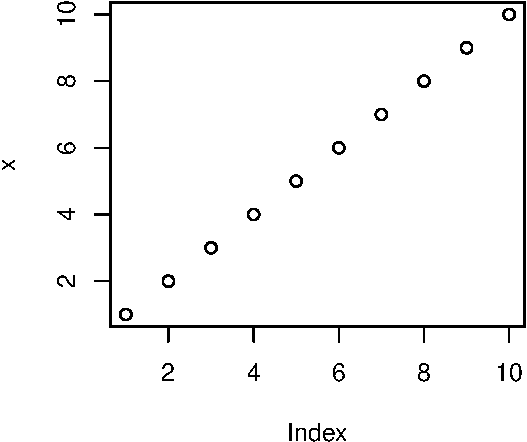
\includegraphics{paper_BiocF1000_files/figure-latex/plot-1.pdf}
\caption{\label{fig:plot}A caption to our sample plot.}
\end{figure}

\subsection{Tables}\label{tables}

Markdown syntax tends to lack some of the more sophisticated formatting
features available in LaTeX, so you may need to edit the tables later to
get the desired format.

\begin{table}[htbp]
\caption{Caption to table.}
\centering
\begin{tabledata}{@{}lll@{}}
\header First name & Last Name & Grade\\
\row John & Doe & 7.5\\
\row Richard & Miles & 2\\
\end{tabledata}
\end{table}

Just like figures, tables with captions will also be numbered and can be
referenced. Captions are entered as a paragraph beginning with the
string ``Table:'' (or just ``:''), which may appear either before or
after the table. A label for the table should appear in the beginning of
the caption in the form of \texttt{(\textbackslash{}\#tab:label)}, e.g.,
see Table \ref{tab:table}.

\begin{table}[htbp]
\caption{\label{tab:table} A table with text justification.}
\centering
\begin{tabledata}{@{}lcr@{}}
\header First name & Last Name & Grade\\
\row John & Doe & 7.5\\
\row Richard & Miles & 2\\
\end{tabledata}
\end{table}

\subsection{Figures}\label{figures}

You can include static figures (i.e.~no generated by code) using the
\texttt{include\_graphics()} function from the \textbf{knitr} package,
in a standard code chunk.

\begin{Shaded}
\begin{Highlighting}[]
\NormalTok{knitr}\OperatorTok{::}\KeywordTok{include_graphics}\NormalTok{(}\StringTok{'frog.jpg'}\NormalTok{)}
\end{Highlighting}
\end{Shaded}

\begin{figure}

{\centering 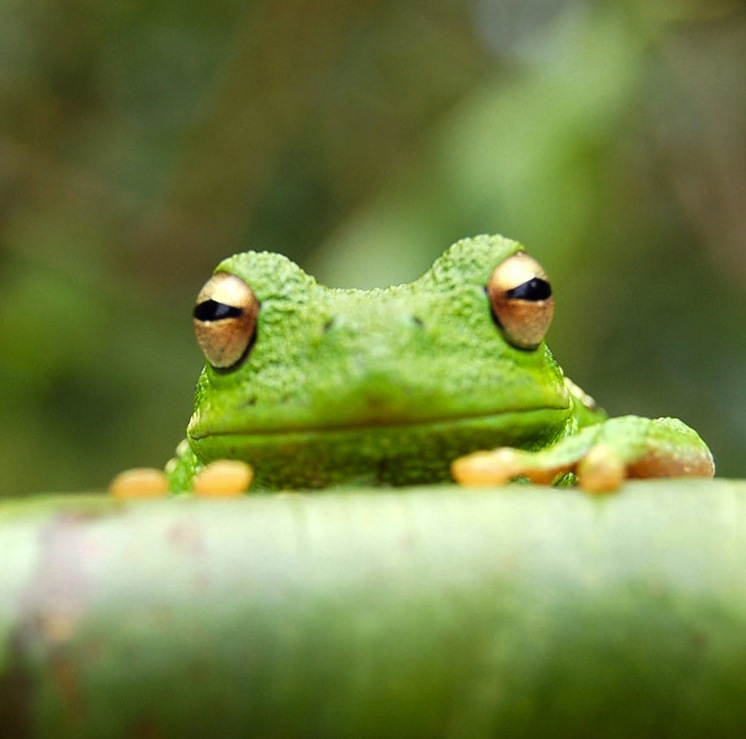
\includegraphics[width=0.5\linewidth]{frog} 

}

\caption{Your figure legend goes here; it should be succinct, while still explaining all symbols and abbreviations.}\label{fig:frog-picture}
\end{figure}

You can again use the \texttt{fig.cap} option to provide the figure
caption, and reference the image based on the code chunk label. You can
also use options such as \texttt{fig.align} and \texttt{fig.width} to
adjust the position and size of the image within the final document,
e.g.~Figure \ref{fig:frog-picture} is a frog.

Alternatively, you can use the standard markdown syntax like so:

\begin{figure}
\centering
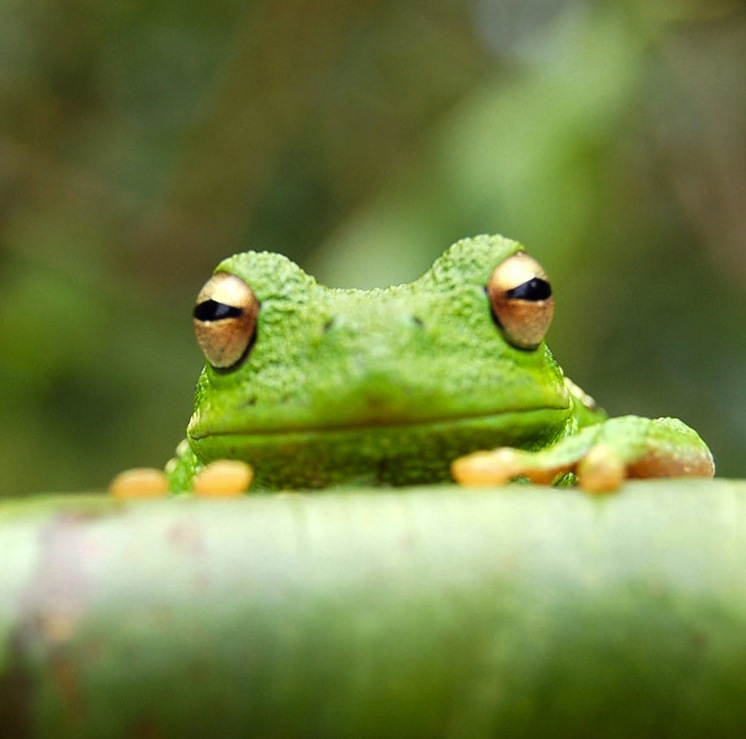
\includegraphics[width=0.25000\textwidth]{frog.jpg}
\caption{This is a smaller version of the same picture, inserted using
the standard markdown syntax}
\end{figure}

Please give figures appropriate filenames, e.g.: figure1.pdf,
figure2.png.

Figure legends should briefly describe the key messages of the figure
such that the figure can stand alone from the main text. However, all
figures should also be discussed in the article text. Each legend should
have a concise title of no more than 15 words. The legend itself should
be succinct, while still explaining all symbols and abbreviations. Avoid
lengthy descriptions of methods.

For any figures reproduced from another publication (as long as
appropriate permission has been obtained from the copyright holder
---see under the heading `Submission'), please include a line in the
legend to state that: `This figure has been reproduced with kind
permission from {[}include original publication citation{]}'.

\subsection{Mathematics}\label{mathematics}

You can use LaTeX syntax to typeset mathematical expressions. Let
\(X_1, X_2, \ldots, X_n\) be a sequence of independent and identically
distributed random variables with \(\text{E}[X_i] = \mu\) and
\(\text{Var}[X_i] = \sigma^2 < \infty\), and let
\[S_n = \frac{X_1 + X_2 + \cdots + X_n}{n}
      = \frac{1}{n}\sum_{i}^{n} X_i\] denote their mean. Then as \(n\)
approaches infinity, the random variables \(\sqrt{n}(S_n - \mu)\)
converge in distribution to a normal \(\mathcal{N}(0, \sigma^2)\).

To number and refer to equations, put them in the equation environments
and assign labels to them, as for Equation \eqref{eq:binom}.

\begin{equation}
  f\left(k\right) = \binom{n}{k} p^k\left(1-p\right)^{n-k}
  \label{eq:binom}
\end{equation}

\subsection{Lists}\label{lists}

You can make ordered lists

\begin{enumerate}
\def\labelenumi{\arabic{enumi}.}
\item
  Like this,
\item
  and like this.
\end{enumerate}

or bullet points

\begin{itemize}
\item
  Like this,
\item
  and like this.

  \begin{itemize}
  \item
    Use indentation

    \begin{itemize}
    \item
      for sub-items
    \end{itemize}
  \end{itemize}
\end{itemize}

\end{document}
